\documentclass[../main.tex]{subfiles}

\begin{document}
\section{Simulation}
\subsection{Numerical setup}\label{sec:numerical}
The 2D incompressible Navier Stokes equations are forced in a periodic domain of size $2\pi \times 2\pi$ with a forcing term that is located in a disk of radius $\pi/k_r$ centered at the origin. The range of values for the parameter $k_r$ is taken to be $\{8, 16, 32, 64\}$ and in all the cases the size of the vortices, which is controlled by $k_\ell$, is set to $k_\ell = 4 k_r$. The $k_r$ being one of those values, represents how smaller is the perturbation region (in diameter) compared to the domain size ($2\pi$). The other parameter $k_\ell$ accounts for the number of vortices introduced in the domain, where there are no other vortices travelling in the domain. In those conditions, $(\pi k_\ell^2)/(\pi k_r^2) = 16$ vortices are introduced in the domain (see figure \ref{fig:forcing}).

\begin{figure}[ht]
	\centering
	\begin{subfigure}{0.45\textwidth}
		\centering
		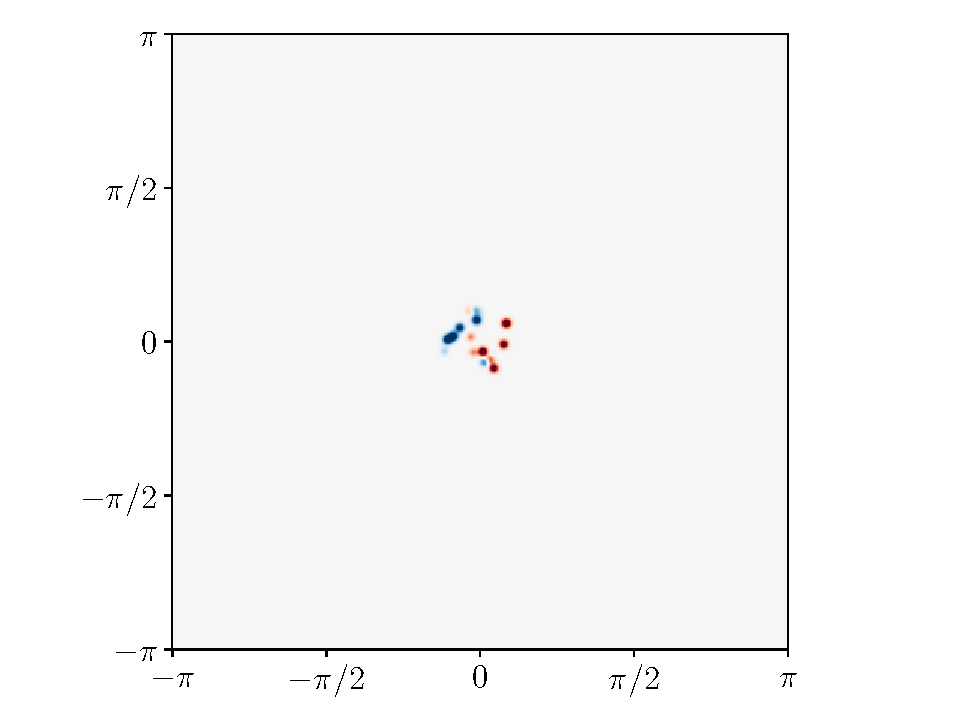
\includegraphics[width=\textwidth]{images/forcing32_8.pdf}
		\caption{$k_r = 8$}
	\end{subfigure}\hspace{0.033\textwidth}
	\begin{subfigure}{0.45\textwidth}
		\centering
		\includegraphics[width=\textwidth]{images/forcing_8.pdf}
		\caption{$k_r = 64$}
	\end{subfigure}
	\caption{Forcing term for different values of $k_r$}
	\label{fig:forcing}
\end{figure}

Recordar afegir dt constant embarrassingly paralllel

\begin{table}[ht]
	\centering
	\def\tickgreen{\textcolor{color_green3}{\ding{51}}}
	\def\tickblue{\textcolor{color_blue3}{\ding{51}}}
	% set space between columns
	\setlength{\tabcolsep}{5pt}
	% set space between rows
	\renewcommand{\arraystretch}{1.5}
	\begin{tabular}{c|cccccccccc}
		\diagbox[width=\dimexpr \textwidth/16+2\tabcolsep\relax, height=1cm]{$k_r$}{$\Re$} & 0.25             & 0.5              & 1                & 2                         & 4                          & 8                          & 16                         & 32                         & 64                & 128               \\
		\hline
		8                                                                                  & \tickgreen_{512} & \tickgreen_{512} & \tickgreen_{512} & \tickgreen\tickblue_{512} & \tickgreen\tickblue_{1024} & \tickgreen\tickblue_{1024} & \tickgreen\tickblue_{1024} & \tickgreen\tickblue_{2048} & \tickgreen_{2048} & \tickgreen_{4096} \\
		16                                                                                 &                  &                  &                  & \tickblue_{1024}          & \tickblue_{2048}           & \tickgreen\tickblue_{2048} & \tickgreen\tickblue_{2048} & \tickgreen\tickblue_{2048} & \tickgreen_{4096} & \tickgreen_{4096} \\
		32                                                                                 &                  &                  &                  & \tickblue_{2048}          & \tickblue_{4096}           & \tickgreen\tickblue_{4096} & \tickgreen\tickblue_{4096} & \tickgreen\tickblue_{4096} & \tickgreen_{8192} & \tickgreen_{8192} \\
		64                                                                                 &                  &                  &                  &                           &                            & \tickgreen_{8192}          & \tickgreen_{8192}          & \tickgreen_{8192}          &                   &                   \\
	\end{tabular}
	\caption{Simulations performed during the project varying the Reynolds number and the forcing parameter $k_r$. The green check mark symbols indicate the simulations done in parallel, splitting the domain between different cores. The blue check mark symbols indicate the simulations done in embarrassingly parallel, where each simulation is done in a single but in many cores at the same time in order to produce statistics results. In each cell, the number indicates the resolution in each dimension employed, which have been proved (a posteriori) to be enough to well-resolve the system.}
	\label{tab:simulations}
\end{table}

All the codes and data used for the simulations are available in the following repository \url{https://github.com/victorballester7/final-master-thesis} (accessed on June 30, 2024).

\subsection{Results}\label{sec:results}
\end{document}
